\chapter{Entity Resolution}

Following schema matching, the next challenge consists of identifying records that refer to the same real-world restaurant across different platforms. Since Google Places, Tripadvisor and TheFork use independent identifiers and maintain separate data repositories, no direct integration key exists. Consequently, entity resolution was implemented as a dedicated record-linkage process~\cite{christen-2012} designed to identify matching restaurants while minimizing both false positives and false negatives.

The entity resolution workflow operates on the clean collections generated during the transformation phase. Google Places was selected as the anchor source due to its superior geographic coverage, high data quality score, and complete coordinate availability. Candidate matches are therefore generated only between Google and Tripadvisor records and between Google and TheFork records. Direct Tripadvisor--TheFork matching is intentionally avoided because both platforms exhibit lower coverage and are expected to be linked indirectly through Google.

\begin{figure*}[t]
    \centering
    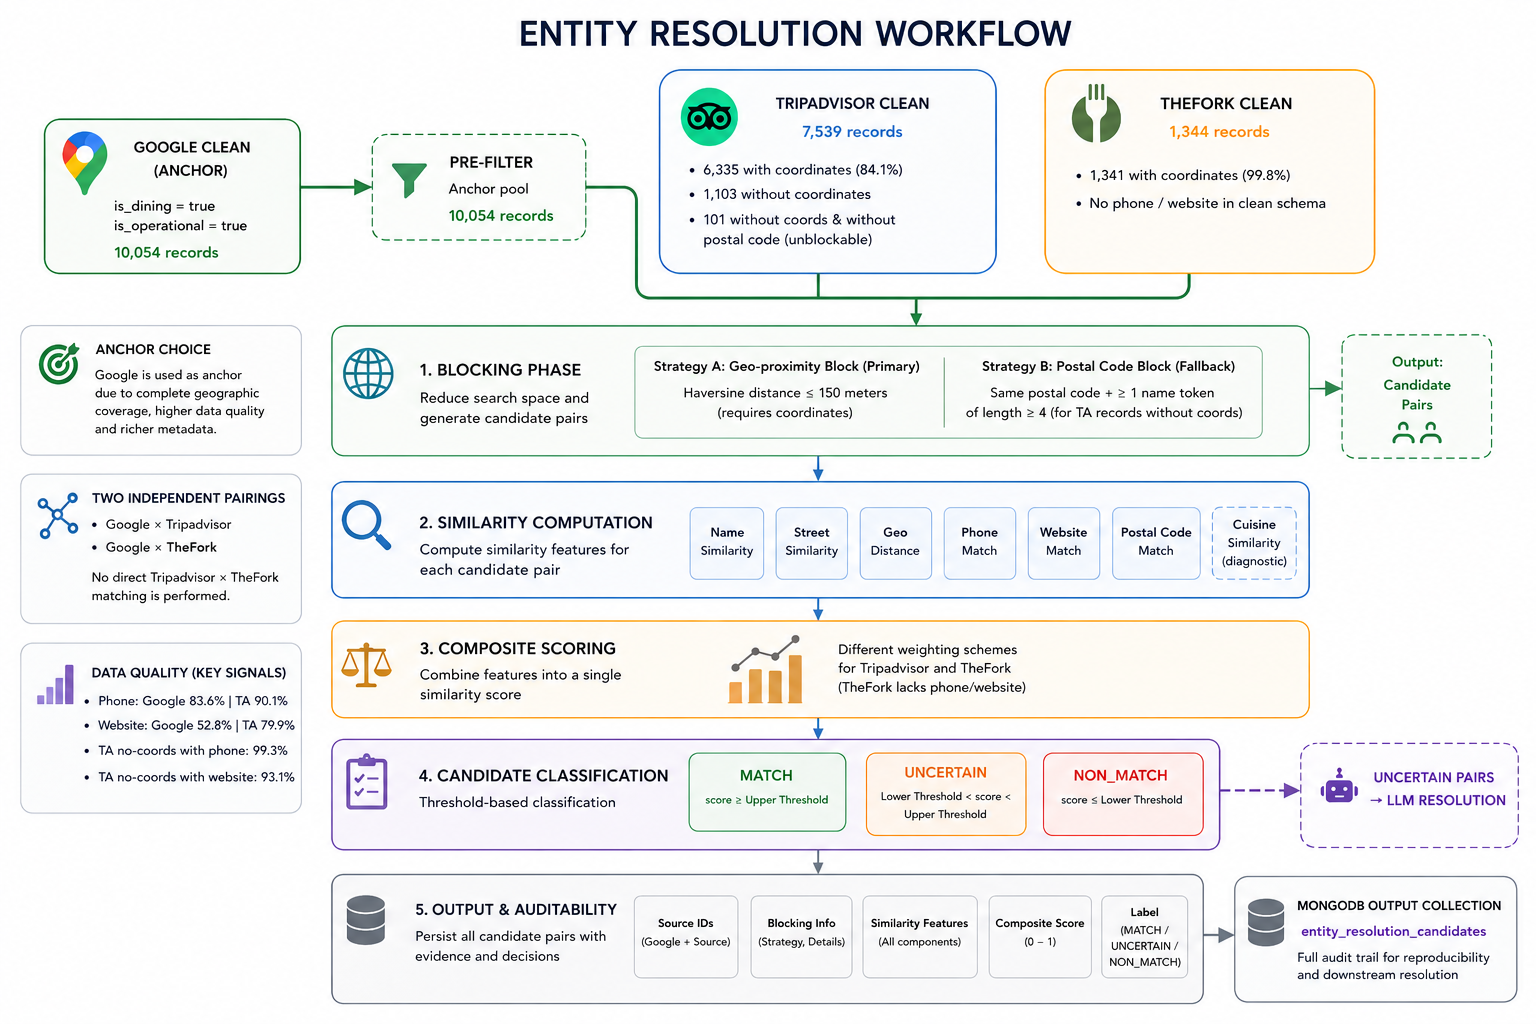
\includegraphics[width=\textwidth]{images/entity_resolution_workflow.png}
    \caption{Entity resolution workflow adopted for restaurant linkage across Google Places, Tripadvisor and TheFork. Google acts as the anchor dataset, candidate pairs are generated through blocking strategies, evaluated using similarity features, and classified into MATCH, NON\_MATCH, or UNCERTAIN categories. Uncertain pairs are forwarded to a subsequent LLM-based resolution stage.}
    \label{fig:entity-resolution-workflow}
\end{figure*}

\section{Blocking Strategy}

A naïve comparison between all records would require evaluating millions of candidate pairs, making the process computationally inefficient. To reduce the search space, a blocking phase was introduced before similarity computation.

The primary blocking strategy is based on geographic proximity. For records containing valid coordinates, candidate pairs are generated only when the distance between the Google restaurant and the corresponding Tripadvisor or TheFork restaurant is below 150 meters. Geographic distance is computed using the Haversine formula, which provides an accurate estimate of distance between two latitude--longitude pairs.

A secondary blocking strategy is applied only to Tripadvisor records that lack geographic coordinates. In this case, candidate pairs are generated when restaurants share the same postal code and at least one common name token of four or more characters. This additional constraint prevents excessively large postal-code blocks from generating an impractical number of comparisons while preserving a high probability of capturing true matches.

Records lacking both coordinates and postal-code information cannot be reliably compared using any available blocking key. These records are therefore explicitly marked as \texttt{UNBLOCKABLE} and preserved for auditing purposes.

\section{Similarity Computation}

For each candidate pair generated during the blocking phase, a set of similarity features is computed. The most important signal is restaurant-name similarity, obtained through token-based fuzzy matching implemented with RapidFuzz after additional normalization steps such as abbreviation expansion, punctuation removal, and whitespace standardization~\cite{rapidfuzz-geopy}.

Additional comparison features include street-name similarity, postal-code agreement, geographic distance, phone-number equality, and website equality when such information is available. Phone numbers and websites are particularly valuable for Tripadvisor matching because they provide strong evidence of identity when identical values are observed across sources.

Cuisine information is also evaluated through set-based similarity measures. However, due to the vocabulary heterogeneity discussed in the schema matching phase, cuisine similarity is used only as a diagnostic feature and does not directly contribute to the final matching score.

\begin{table*}[t]
\centering
\footnotesize
\begin{tabular}{p{0.28\linewidth}p{0.22\linewidth}p{0.35\linewidth}}
\toprule
\textbf{Feature} & \textbf{Type} & \textbf{Purpose} \\
\midrule
Name similarity & Fuzzy matching & Primary identity signal \\
Street similarity & Fuzzy matching & Address consistency check \\
Geographic distance & Spatial similarity & Distinguishes nearby venues \\
Phone match & Exact match & Strong matching evidence \\
Website match & Exact match & Strong matching evidence \\
Postal-code match & Exact match & Geographic consistency check \\
Cuisine similarity & Diagnostic only & Analytical support feature \\
\bottomrule
\end{tabular}
\caption{Similarity features used during entity resolution.}
\label{tab:er-features}
\end{table*}

\section{Candidate Classification}

Similarity features are combined into a weighted composite score representing the likelihood that two records correspond to the same restaurant. Different weighting schemes are adopted for Tripadvisor and TheFork because TheFork does not provide phone numbers or restaurant websites in the clean schema. For Tripadvisor the score weights name similarity at 0.40, geographic proximity at 0.25, phone match at 0.15, street similarity at 0.10, and website match at 0.10. For TheFork, where contact signals are unavailable, the weight is redistributed over the remaining features, namely name similarity at 0.50, geographic proximity at 0.35, and street similarity at 0.15. In both cases name similarity is the dominant identity signal, complemented by geographic proximity.

The resulting score is compared against two calibrated thresholds. Candidate pairs with scores above the upper threshold are automatically classified as \texttt{MATCH}, while pairs below the lower threshold are classified as \texttt{NON\_MATCH}. Records falling between the two thresholds are assigned to an intermediate \texttt{UNCERTAIN} category.

\begin{table*}[t]
\centering
\footnotesize
\begin{tabular}{p{0.32\linewidth}cc}
\toprule
\textbf{Candidate type} & \textbf{Lower threshold} & \textbf{Upper threshold} \\
\midrule
Tripadvisor, non-chain venues & 0.58 & 0.63 \\
TheFork, non-chain venues & 0.86 & 0.94 \\
Tripadvisor, chain venues & 0.49 & 0.52 \\
TheFork, chain venues & 0.76 & 0.79 \\
\bottomrule
\end{tabular}
\caption{Calibrated entity-resolution thresholds used for automatic candidate classification.}
\label{tab:er-thresholds}
\end{table*}

Thresholds were calibrated from manually labelled candidate samples. Normal venues and chain venues were treated separately because repeated brands, such as fast-food or casual dining chains, require stricter branch-level evidence than independent restaurants. The calibration files are kept as reproducible gold-standard artifacts and are not used as hidden runtime inputs by the entity-resolution command.

This three-way classification strategy was intentionally adopted to reduce the risk of incorrect automatic decisions. Rather than forcing all pairs into a binary outcome, ambiguous cases are isolated and delegated to a subsequent resolution stage.

An additional fast-path mechanism is implemented for Tripadvisor records without coordinates. When phone numbers or websites are identical across sources, the candidate pair can be classified as a \texttt{MATCH} without requiring further similarity computation, subject to the conservative chain-handling rules described below. This optimization significantly improves both efficiency and precision because identical contact information provides strong evidence that two records refer to the same establishment.

\subsection{Chain and Franchise Handling}

Restaurant chains and franchises require a dedicated matching strategy because the
usual identity signals become unreliable when the same brand operates several
branches in Milan. Two different branches of the same franchise, such as two
\textit{KFC}, \textit{Poke House}, or \textit{McDonald's} venues, share almost
identical names and often the same corporate website, yet they are distinct
real-world restaurants. The guiding principle is therefore that \emph{the same
brand does not imply the same venue}: for chain candidates, name and website
similarity are no longer sufficient evidence of a match, and branch-level evidence
is required instead.

Chain candidates are first identified through brand detection. A curated list of
chain brands observed among the repeated Google anchor names in the Milan dataset
(for example \textit{KFC}, \textit{Poke House}, \textit{McDonald's},
\textit{Five Guys}, \textit{Spontini}, \textit{Starbucks}, and \textit{Roadhouse})
is matched against the normalized restaurant name. Generic repeated names that do
not identify a specific brand, such as \textit{bar} or \textit{pizzeria}, are
deliberately excluded. A candidate pair is flagged as a chain when either the
Google record or the source record carries a recognized brand.

Chain candidates are then subject to two hardening rules on top of the stricter
calibrated thresholds already reported in Table~\ref{tab:er-thresholds}. First, the
website fast-path is suppressed for chains: because all branches of a franchise
typically expose the same corporate website, website equality is not accepted as
proof of identity, while the more branch-specific phone fast-path remains valid.
Second, a chain pair that would otherwise be classified as \texttt{MATCH} is
downgraded to \texttt{UNCERTAIN} when no geographic evidence is available, or when
the two venues are farther apart than a small automatic-match radius (75~m by
default). This ensures that automatic chain matches are only accepted when the two
records are geographically compatible with being the same branch. Every hardening
decision is recorded in a \texttt{chain\_hardening} field, so the more conservative
treatment of franchises remains fully auditable.

\section{Output and Auditability}

The output of the entity resolution process is stored in the MongoDB collection \\
\texttt{entity\_resolution\_candidates}. Each candidate pair preserves the identifiers of both source records, the blocking strategy used to generate the candidate, the individual similarity components, the composite score, and the final classification label.

Maintaining both positive and negative decisions provides a complete audit trail of the matching process. Furthermore, uncertain candidates are retained together with all supporting evidence, enabling a subsequent large-language-model resolution step without requiring candidate generation to be repeated.

The resulting collection therefore acts as the bridge between schema-level integration and the construction of the final integrated restaurant dataset, providing a transparent and reproducible record-linkage layer for the entire project.

\section{Threshold Calibration}

The decision thresholds were calibrated against a manually labelled gold standard. The gold standard was constructed by sampling candidate pairs generated during blocking and exporting each of them together with its full matching evidence, including the two restaurant names, addresses, coordinates, the individual similarity components, and the automatic label produced by the pipeline. Each sampled pair was then reviewed by hand and assigned a human label of \texttt{MATCH} or \texttt{NON\_MATCH}, giving a ground truth against which the automatic decisions can be compared.

Two disjoint gold subsets were used, following a calibrate-then-verify protocol. The calibration subset contains 600 labelled candidate rows, split between normal venues and chain venues, and is used exclusively to choose the lower and upper decision thresholds ($d_{\min}$ and $d_{\max}$) reported in Table~\ref{tab:er-thresholds}. Because the thresholds are fitted on this subset, its metrics alone would be an optimistic estimate of quality. For this reason a second, additional set of candidate pairs was hand-labelled purely for verification: a separate out-of-sample (holdout) subset of 288 rows, obtained after de-duplication and after excluding any candidate already present in the calibration files. This holdout is never used to choose $d_{\min}$ or $d_{\max}$; it only verifies the already-calibrated thresholds, providing an unbiased estimate of how the classifier behaves on unseen pairs. The classifier error on this holdout, together with one-to-one link survival and Tripadvisor geocoding accuracy, is reported as part of the post-integration quality assessment in Section~\ref{sec:post-integration-quality}.

\section{LLM based labelling on Uncertain Pairs}

While the deterministic entity resolution process is able to automatically classify the majority of candidate pairs as either \texttt{MATCH} or \texttt{NON\_MATCH}, a subset of cases remains inherently ambiguous. These candidate pairs fall within the intermediate decision region defined by the three-way classification policy and are labelled as \texttt{UNCERTAIN}. Rather than forcing a potentially unreliable automatic decision, the implemented pipeline provides an optional second adjudication layer based on a Large Language Model (LLM), applied exclusively to these unresolved cases.

The LLM component does not replace the deterministic record linkage process and does not operate on the full space of possible source combinations. Instead, it acts as a controlled semantic reasoning layer on top of the candidate pairs already generated through blocking and similarity scoring. Consequently, the computational cost and decision scope remain limited to a relatively small set of ambiguous records. Only documents in the collection \texttt{entity\_resolution\_candidates} with \texttt{label = UNCERTAIN} and no previous LLM decision are considered for processing.

Candidate pairs are grouped according to the source record identifier, so that the model evaluates a single Tripadvisor or TheFork restaurant together with its competing Google candidates rather than examining pairs independently. For each group, Google candidates are ranked according to their deterministic score, geographic proximity, name similarity, and street similarity. The prompt then presents the source restaurant together with the highest-ranked candidates and all relevant matching evidence, including names, addresses, coordinates, contact information, ratings, cuisine descriptors, and similarity components.

The model is instructed to select one of three possible outcomes: \texttt{MATCH}, when exactly one candidate can be confidently identified as the same physical restaurant; \texttt{NON\_MATCH}, when none of the candidates appear plausible; or \texttt{UNCERTAIN}, when the available evidence is insufficient or multiple candidates remain equally plausible. To ensure reproducibility and machine-readable outputs, responses are constrained to a predefined JSON schema containing the final decision, the selected candidate identifier, a confidence value, a textual explanation, and a set of predefined risk flags describing potential sources of ambiguity.

A key design principle of the implemented approach is that LLM decisions are never accepted blindly. Every response is subjected to a deterministic post-validation policy before being incorporated into the integration workflow. Candidate matches may be downgraded from \texttt{MATCH} to \texttt{UNCERTAIN} when the confidence value falls below a configurable threshold, when the selected candidate does not belong to the candidate set presented in the prompt, when severe risk flags are detected, or when geographic evidence is inconsistent with the absence of supporting contact information. This validation layer ensures that the generative component remains subordinate to conservative and transparent decision rules.

The resulting decision is stored as an additional layer of metadata rather than replacing the original deterministic classification. Fields such as \texttt{llm\_label}, \texttt{llm\_confidence}, \texttt{llm\_reason}, \texttt{llm\_risk\_flags}, and \texttt{llm\_prompt\_version} are persisted together with the original similarity evidence, enabling full traceability of the adjudication process. The downstream unification command consumes \texttt{llm\_label} when it is available; otherwise, it falls back to the deterministic label. Consequently, deterministic matches remain valid, uncertain pairs promoted by the LLM can contribute to the final integrated dataset and unresolved ambiguities remain excluded from automatic integration.
